\documentclass[12pt,a4paper]{article}
\usepackage{fullpage}
\usepackage{fancyhdr} %headers
\usepackage{titlesec}
\usepackage{graphicx} %images
\usepackage{amsmath} %maths
\usepackage{amssymb} %maths symbols
\usepackage{subfig}
\usepackage[section]{placeins}
\usepackage{listings}
\usepackage[T1]{fontenc}
\usepackage{lastpage}

\usepackage{enumerate}

\usepackage{braket}

\renewcommand{\headrulewidth}{0pt}

\renewcommand\thesubsection{\arabic{subsection}}

\nonstopmode

\setlength{\headheight}{15pt}

\graphicspath{ {img/} }

%\titleformat{name=\section}
%  {\normalfont\scshape}{\thesection}{1em}{\large}

\titleformat{name=\section}
  {\normalfont\large\scshape}{\thesection}{1em}{}

\titleformat{name=\subsection}
    {\normalfont\normalsize}{\thesubsection}{1em}{\large}

%%\titleformat{\subsubsection}
%  {\normalfont\normalsize}{\thesubsubsection}{1em}{}

\setlength{\parindent}{0em}
\addtolength{\parskip}{1ex}

\lstset{
	basicstyle=\scriptsize,
	breaklines=true
}

\pagestyle{fancy}
\setlength{\headsep}{0.2in}
\title{Testing the Performance Limitations of Simulating a Network of Database Nodes on One Machine}
\author{Alex Bostock}

\date{}
\fancyhf{}
%\lhead{Summer Work IB/II}
%\rhead{atb46}

\cfoot{\thepage / \pageref{LastPage}}

\begin{document}
\maketitle
\thispagestyle{fancy}

\section*{Methodology}

I have implemented a simple network simulator, as described in my design specification. I used this system to test what throughput of transactions my system can achieve, particularly when each transaction involves concurrent disk I/O by many simulated nodes.

I ran tests based on $90\%$ read transactions and $10\%$ writes. For each read transaction, I had every node in the system concurrently read a file. For each write transaction, I had every node concurrently read a file then write a file. This emulates how quorum assembly works, with many nodes doing the same work for each transaction. Having every node execute every transaction makes this an upper bound. Only a subset of the nodes will be involved in each transaction, depending on quorum sizes. I ran these tests with varying transaction rates and varying numbers of nodes.

I measured the throughput of the system as number of transactions completed divided by total execution time. I also calculated node throughput: the product of throughput and the number of nodes. These tests showed that the number of nodes did not affect node throughput. The node throughput is the rate at which disk operations are completed. Since my machine has 1 disk, all disk operations are sequential. Go can efficiently schedule many concurrent routines waiting for disk operations, so only the total number of disk operations affects the result.

This test also showed how node throughput increases as rate of transactions increases. At a low rate of transactions (eg. 10 transactions per second, 1000 nodes), node throughput is very close to transaction rate, so every transaction is being processed in real time. At higher rates of transactions, the node throughput reached a constant limit, around 30000 transactions per second. This is where disk I/O is the bottleneck on throughput.

I then ran further tests to determine the maximum throughput given different size values being read from and written to disk. Since the number of nodes does not affect node throughput, I ran every test with 1000 nodes, and tested several high rates of transactions. By testing multiple different rates and verifying that each provides a similar result, I can be confident that the rate was high enough to reach the disk bottleneck in each case.

I repeated this test using a variant on the system where only write transactions would involve disk access, to simulate performance if all read transactions were served from an in-memory cache. I also repeated the two tests on a remote Digital Ocean server, to test for any performance difference between different machines.

\begin{figure}
  \centering
    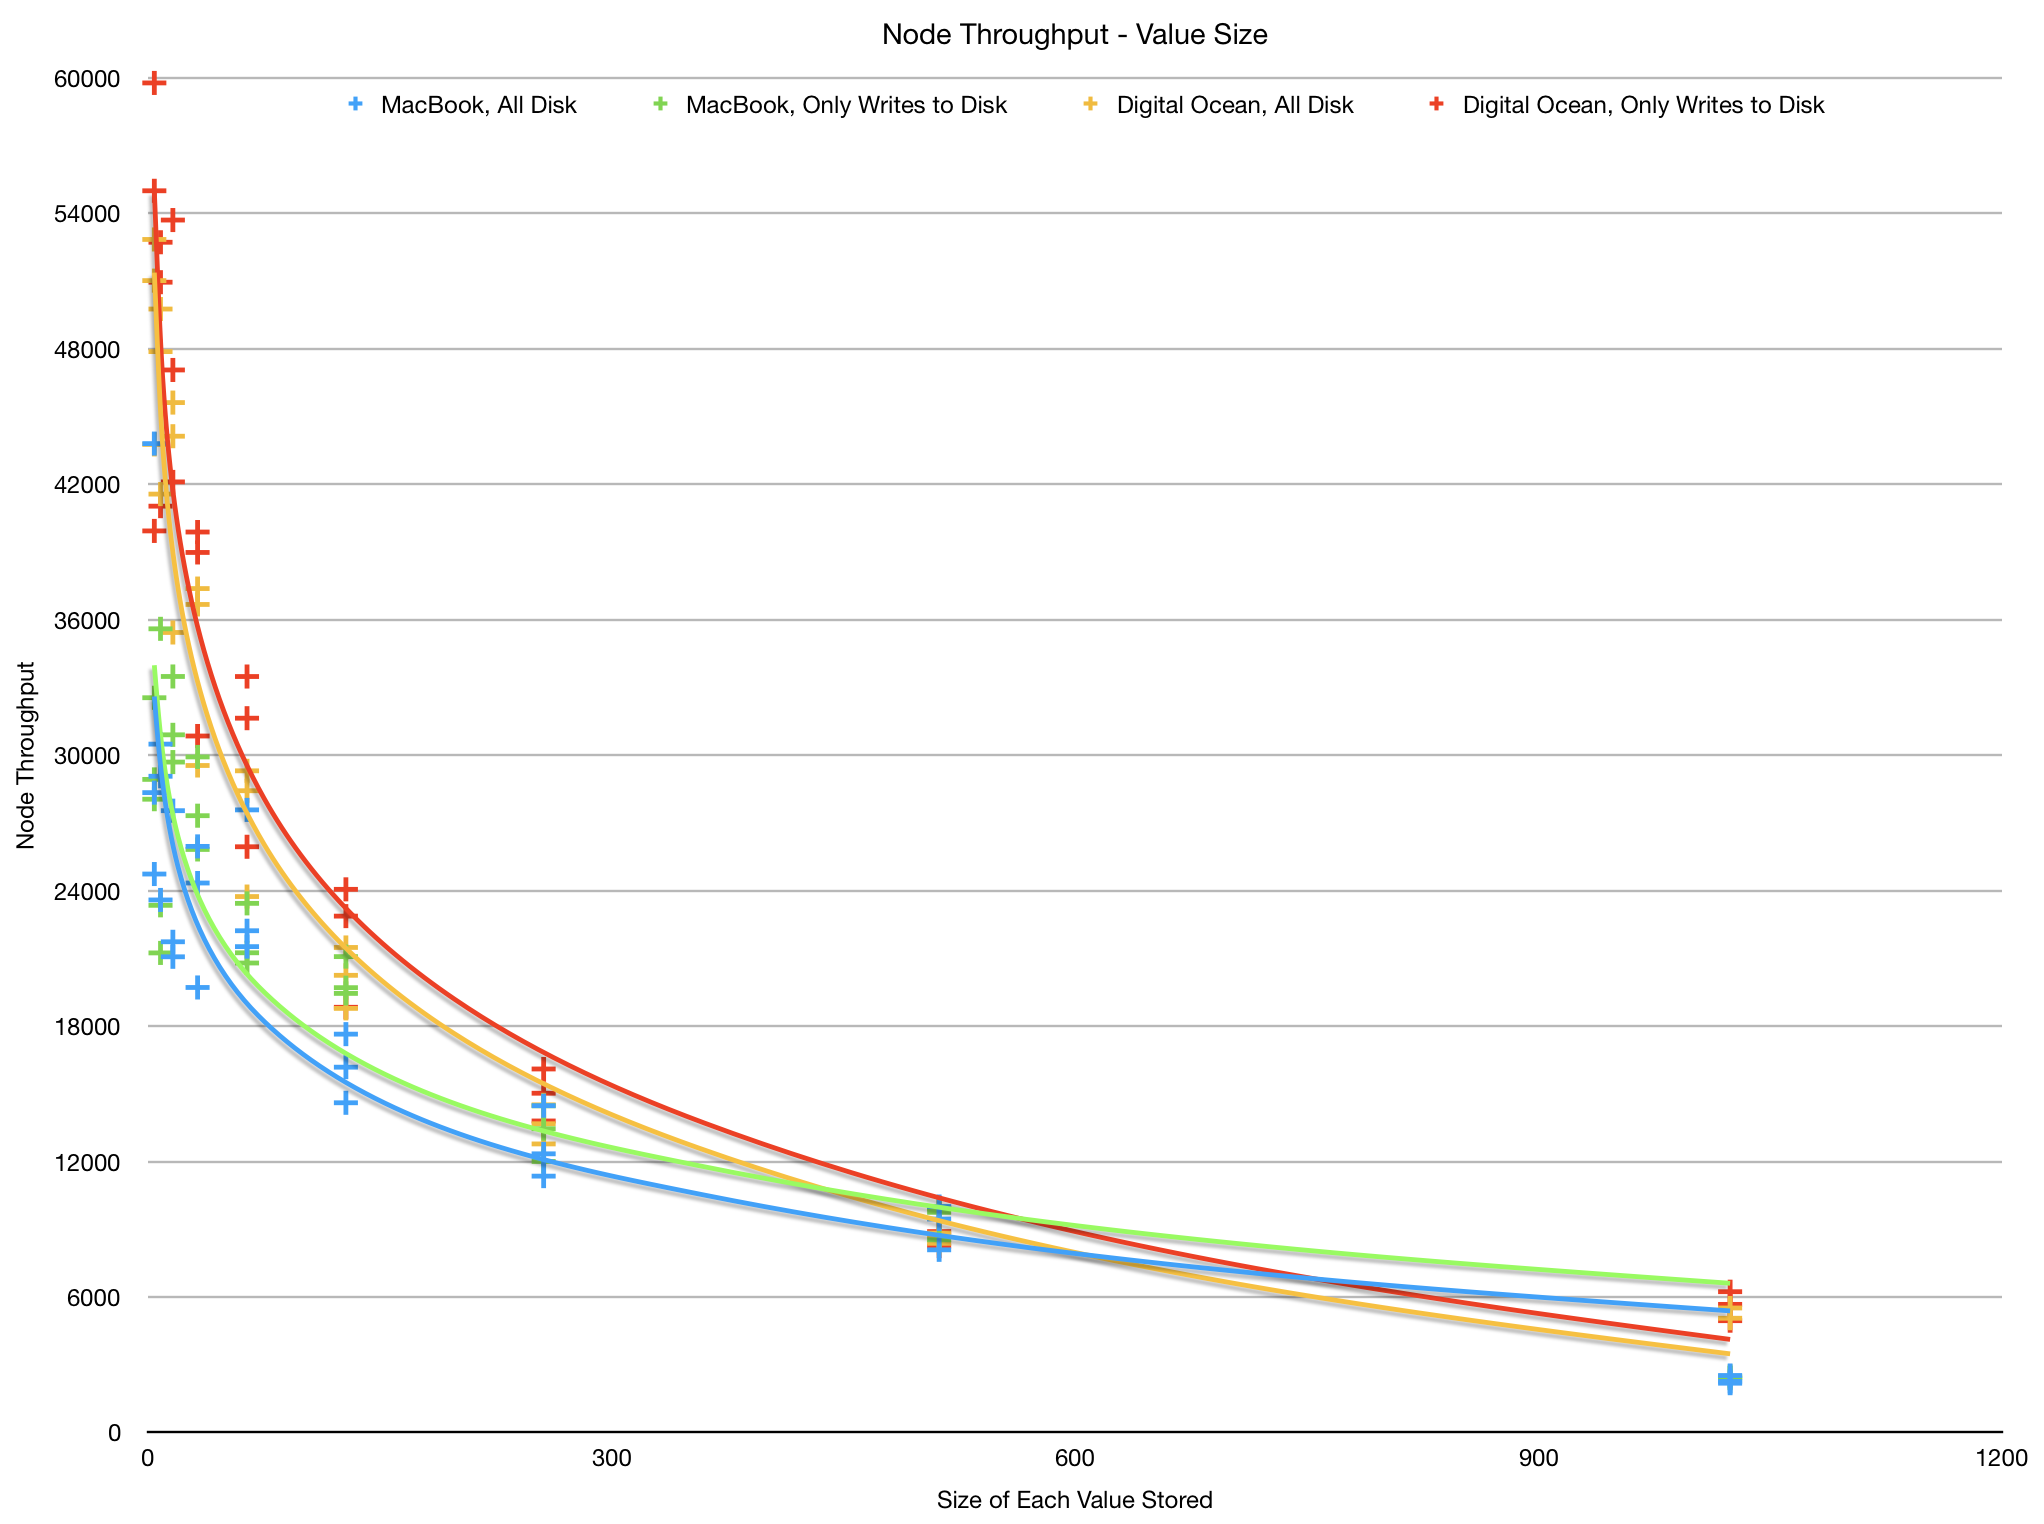
\includegraphics[width=1\textwidth]{figure}
  \caption{Results of running throughput tests on two different machines, varying the size of data values being read from and written to disk. In each test, $90\%$ of transactions were reads and $10\%$ were writes, and every transaction was concurrently sent to each of $1000$ nodes, all running on the same machine. For All Disk tests, each node read a file for each read transaction, and read a file then wrote a file for each write transaction. For Only Write to Disk tests, nodes did the same for write transactions, and no work for reads. The size of each file in bytes is varied on the $x$-axis. The value measured for each test is node throughput: number of nodes * number of transactions / total time taken in seconds.}
\end{figure}

\section*{Implications}

For this project, I want to evaluate 3 key things:

\begin{itemize}
  \item
  Verify that the system provides the correct consistency guarantees under all conditions, especially with the strongly consistent variant.

  \item
  Measure maximum throughput of transactions the system can handle.

  \item
  Measure the time to reach consistency in the eventually consistent variant.

\end{itemize}

In order to measure maximum throughput, I need to test the system with a high rate of transactions, high enough that the system reaches a bottleneck which prevents throughput increases to match demand. I need to make sure that the bottleneck it reaches is a limitation of the system design, not of my experimental setup.

I expect that the throughput limit in my system design depends on network latency. I need to make sure that the system reaches a network I/O bottleneck before it reaches a disk I/O bottleneck due to running on a single machine, with a single disk.

I will assume that each transaction involves reading or writing a $256$ byte file, on each node involved in the transaction. This has to include, as a minimum, a key, a value and a Lamport timestamp. Suppose each value is a tweet (around $140$ bytes). Each timestamp is $8$ bytes (according to my design). So $256$ bytes should be adequate to store one key-value pair and its timestamp. While my design specification says store multiple values in each file, changing this to one key-value pair per file would be a minor change.

According to my experiment, with $256$ byte values, $15000$ disk operations per second is achievable (assuming $10\%$ of transactions are writes). I want to be able to test the system with $1000$ nodes.

Assume that a read transaction involves a network message, a disk operation, then another network message. Also assume that the network latency and disk latency are constants $t_n$ and $t_d$, respectively, so the time for $1$ transaction should be $2t_n + t_d$.

In the worst case, every node will be accessing the disk at the same time. Using a single machine with a single disk, when every node tries to access the disk simultaneously, $1$ node will have to wait for the other $999$ nodes to access the disk before it can continue. That node will take time $2t_n + 1000t_d$ to complete a transaction. With quorum assembly, a transaction cannot complete until every node involved has responded, so the time taken is the maximum time taken by any node involved.

This means that the absolute error in transaction time in the worst case is $(2t_n + 1000t_d) - (2t_n + t_d) = 999t_d$. The relative error is $\frac{999t_d}{2t_n + t_d}$.

Assume that $t_n$ is $20$ milliseconds, and $t_d = \frac{1}{15000}$ seconds (based on my experiment). This means the error rate is:

$$\frac{\frac{999}{15000}}{\frac{40}{1000} + \frac{1}{15000}} = \frac{999}{601} \approx 166\%$$

This is not good enough.

\section*{Possible Solutions}

\subsection{Use multiple machines}

This would require changes to the test framework design, and ideally very fast \& reliable networking.

I could use Digital Ocean, with fast networking between nodes in the same data centre. This should minimise latency and variance of latency from the real world, so I can still add simulated latency with minimal noise.

Or explore alternative resources for running multiple networked machines with minimal latency.

Cost: more work to build, and very reliant on external resources.

\subsection{Store data in memory instead of disk}

In addition to the persistent data store described in my design, I could build an alternative store, which stores data in memory. This should be simple to build. I could still use the persistent store to test correctness of the system, but use the in-memory store for high intensity performance tests.

The key limitation of this approach is how much data can be stored in memory, For example, with $1000$ nodes, each storing $2$ MB, the system would be using $2$ GB of memory. This is not a major problem. My system is mainly concerned with testing consistency properties when the same values are modified repeatedly, rather than storing high volumes of data.

\end{document}
